\paragraph{Comunicaciones inalámbricas}

Implementar un bus de comunicación eficiente (por ejemplo, CAN, Ethernet) para conectar los diferentes módulos del robot. Garantizar que la comunicación sea robusta y de baja latencia.

\paragraph{Microcontroladores}

Dividir el procesamiento en subsistemas especializados:
    Procesamiento de Sensores: Fusión de datos, localización y mapeo (SLAM).
    Planificación y Navegación: Algoritmos de planificación de rutas y evitación de obstáculos.
    Control de Movimiento: Algoritmos de control para los actuadores (por ejemplo, control PID).
    Utilizar hardware especializado (como FPGAs o GPUs) para tareas intensivas en cálculo.

% https://docs.espressif.com/projects/esp-idf/en/latest/esp32/api-reference/peripherals/pcnt.html
que necesitamos del microcontrolador? contador de pulsos, interrupciones, comm inalámbricas, muchos puertos, PWM, etc
elegiríamos ESP32 y ESP32-cam
Contador de eventos: Es necesario que tenga un contador de eventos o pulsos. Aparentemente tiene esta funcionalidad de manera nativa. Tiene 8 unidades de conteo con 2 canales cada uno, pudiendo tener 16 fuentes de pulsos. Los contadores tienen un filtro (simil antirrebote) para las señales de entrada. Importante que cada pulso dure por lo menos 12.5ns.

\paragraph{Cámara y streaming de video}

debe poder transmitir imágenes de la cámara a una tasa razonable de FPS. Parece que también soporta esto.

\paragraph{Sensores y actuadores}

Integrar los sensores (cámaras, LiDAR, IMU, etc.) y actuadores (motores, servos, etc.) con interfaces claras hacia la capa de procesamiento.
Garantizar que los datos sensoriales sean preprocesados (por ejemplo, filtrado de ruido) antes de ser enviados a la unidad de control.

\textbf{para odometria:}

Sensor de mouse óptico. Tienen bastante precisión. Se podría hacer para reemplazar los encoder. Se pondrían 2 o más para detectar diferencia en las velocidades de los motores. Por trabajos anteriores no son muy buenos.

\begin{center}
    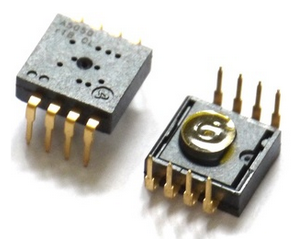
\includegraphics[width=0.25\linewidth]{mt_sensor_optico_mouse}
\end{center}

\textbf{para medidor de RPM:}

encoder rotativo
algun otro que haya

\textbf{para seguidor de linea:}
magneticos, etc

\paragraph{PID}

como se puede controlar la velocidad de un motor?
que formas hay de controlar un motor DC?